\documentclass{article}
\usepackage[utf8]{inputenc}
\usepackage{amsmath}
\usepackage{listings}
\usepackage{geometry}
\usepackage{graphicx}
\usepackage{appendix}
\usepackage{subfig}
\usepackage{gensymb}
\usepackage{cancel}
\usepackage{physics}
\usepackage{empheq}
\usepackage{wrapfig}
\usepackage[colorlinks=true]{hyperref}
\usepackage{xcolor}
\definecolor{codegreen}{rgb}{0,0.6,0}
\definecolor{codegray}{rgb}{0.5,0.5,0.5}
\definecolor{codepurple}{rgb}{0.58,0,0.82}
\definecolor{backcolour}{rgb}{0.95,0.95,0.92}
\lstdefinestyle{mystyle}{
    backgroundcolor=\color{backcolour},   
    commentstyle=\color{codegreen},
    keywordstyle=\color{magenta},
    numberstyle=\tiny\color{codegray},
    stringstyle=\color{codepurple},
    basicstyle=\ttfamily\footnotesize,
    breakatwhitespace=false,         
    breaklines=true,                 
    captionpos=b,                    
    keepspaces=true,                 
    numbers=left,                    
    numbersep=5pt,                  
    showspaces=false,                
    showstringspaces=false,
    showtabs=false,                  
    tabsize=2
}

\lstset{style=mystyle}

\title{Generative Imaging \\
\Large Using Neural Networks to Generate MNIST Digits \\
\small A self study at the University of Oslo \\
\small \href{https://github.com/simloken/Generative_Imaging}{Github repository}}
\author{Simen Løken}
\date{April 2025}

\begin{document}

\maketitle

\newpage
{
  \hypersetup{linkcolor=black}
  \tableofcontents
}
\newpage
\section{Abstract}
This paper introduces a comparative overview of four prominent generative modeling techniques, Restricted Boltzmann Machines (RBMs), Generative Adversarial Networks (GANs), Variational Autoencoders (VAEs) and Denoising Diffusion Probabilistic Models (DDPMs), applied to the task of generating new MNIST digits. We present a concise explanation of the underlying theory and architecture for each method, detailing their unique features and their training procedures. By focusing on the insights on model performance, complexity and image fidelity, this work serves as an accessible primer for those interested in exploring an introduction to generative imaging in practice. Our discussion touches on the relevance of these techniques in the broader scientific space together, with an extra focus on physics applications.
\nocite{foster2019generative}
\nocite{tomczak2022deep}
\nocite{goodfellow2014generativeadversarialnetworks}
\nocite{kingma2022autoencodingvariationalbayes}
\nocite{ho2020denoisingdiffusionprobabilisticmodels}

\newpage
\section{Introduction}
\subsection{Machine Learning and neural networks}
Machine Learning is the idea that we can teach a computer to see patterns that aren't necessarily "visible" to humans. It's a common concept which is widely used when dealing with data that has a high dimensionality. Consider, for example, wanting to predict whether or not a patient has cancer, or is at risk of it. Generally, we'd want tens if not hundreds of different data points for each person. Which data point then contributes the most to a possible cancer diagnosis? Machine learning solves this for us in many very intuitive ways, with many differing methods with their own strengths and weaknesses.
\newline
Neural Networks take this concept a step further. Instead of now purely only looking at (in the example above) high-dimensional pattern recognitions, we now seek to mimic the human brain's inherent ability to recognize patterns and make complex associations. Inspired by biological neurons, artificial neural networks consist of layers of interconnected nodes (or neurons), each performing mathematical operations to transform input data into meaningful outputs.
\newline
At their core, neural networks operate using a system of weights and activations. Each neuron receives inputs, applies a weight to each, sums them up, and then passes the result through an activation function. This activation function introduces non-linearity, allowing the network to learn complex, non-obvious relationships within the data. These networks are typically trained using a process called backpropagation, which adjusts the weights of the neurons to minimize errors in predictions.
\newline
The depth and structure of a neural network significantly impact its capabilities. A simple feedforward neural network consists of an input layer, one or more hidden layers, and an output layer. However, more advanced architectures like convolutional neural networks (CNNs) are specifically designed for image processing, while recurrent neural networks (RNNs) excel at handling sequential data, such as speech and time-series forecasting.
\newline
Neural networks have revolutionized numerous fields, from medical diagnostics and finance to autonomous vehicles and natural language processing. However, their effectiveness depends on factors such as data quality, computational resources, and model architecture. Although neural networks can capture intricate patterns and relationships, they also require careful tuning and large amounts of data to perform optimally.
\subsection{What makes a model generative?}
So what makes a model generative? Non-generative models typically are typically called discriminative and focus on classifying or predicting an outcome, such as classifying a handwritten digit over the possible digits 0-9. Generative models, in contrast, learn to produce new data samples as opposed to just making decisions. We no longer map inputs to outputs but instead learn the probability distribution of the data, allowing us to generate entirely new data points.
\newline
In more mathematical terms, a discriminative network learns the conditional probability $P(y | x)$, where the inputs $x$ are mapped to the labels $y$, whereas a generative model learns the true probability distribution $P(x)$. Drawing then from this distribution, we can generate new samples.
\newpage
\subsection{Generative imaging - why?}
So why generative imaging? Why is it such an important technology? We need only look at the recent emergence and explosion of popular generative image models like DALL-E 3 to see its transformative potential. Generative imaging enables the creation of novel, realistic images by learning from vast datasets, allowing for applications that range from artistic expression to scientific research.
\newline
In the medical field, generative models have been used to improve imaging techniques. For example, this paper \cite{hein2024physicsinspiredgenerativemodelsmedical} discusses how diffusion and Poisson flow models can enhance image reconstruction and analysis, leading to more accurate diagnostics.
\newline
Generative imaging also plays a significant role in physics-related research. The study \cite{Guo_2022} introduces a two-step algorithm that combines known physics with learned data priors to improve tomographic reconstructions, potentially reducing the required radiation dose for imaging. 
\newline
Another example is the development of a physics-driven untrained generative adversarial network for 3D microscopic imaging using digital holography, as detailed in \cite{chen2022dhganphysicsdrivenuntrainedgenerative}. This approach enhances the reconstruction quality of microscopic images without the need for extensive training datasets.
\newline
The examples above are limited to only some applications within the hard sciences, as that is my field, but it goes without saying how much of a useful tool this is even for the everyday layman. It is therefore important to get a more robust understanding of this relatively new technology, which we will do by exploring various different models, and how they generate MNIST digits.
\newpage
\section{Theory and Method}
\subsection{Neural Networks}
Neural Networks are a class of machine learning models that are (as previously mentioned) inspired by the structure and functionality of biologoical neural networks, ie. our brains. They consist therefore of interconnected layers of artificial neurons, processing and learning representations of data. Mathematically, a neural network is a function approximator that learns a mapping
\begin{equation}
    f \; :\; X \xrightarrow{} Y
\end{equation}
by optimizing parameters using a given dataset \newline
A neuron computed a weighted sum of inputs and passes it through an activation function
\begin{equation}
    z = \sum_{i=1}^n w_i x_i + b = \boldsymbol{w}^T \boldsymbol{x} + b
\end{equation}
where $\boldsymbol{x}$ is the input vector, $\boldsymbol{w}$ the weights, $b$ the bias and $z$ the pre-activation output, which we pass through an activation function.
\newline
It is important to note that the activation function is not necessarily the same across all layers of a given network, but is typically chosen with respect to both the model and the type of data, or its range. For example, data that is generally not centered around 0, will perform poorly with an activation function such as $\tanh(z)$, which is zero-centered. We will talk more about activation functions later \ref{acti}, but let us first take a look at our models to get a better understanding of how an activation function impacts a given model.
\subsubsection{The Latent Space}
Before we go any further into the specifics of each model, we should first briefly talk about the latent space, and what it means. We touched on it briefly in the introduction, the idea that we can teach a network to see patterns in data that aren't strictly visible to humans. What is actually meant by this, is that we can extract the "latent space" of the data. The latent space is a compressed, abstract representation of data learned by a neural network. We may then typically take some high-dimensional input data and map it into a lower-dimensional space, the name "latent" coming from the idea that the features in this space are not directly observable, instead hidden representations that capture the underlying factors or features that best describe the data.
\subsection{Models}
While many modern generative methods rely on deep learning frameworks like Generative Adversarial Networks (GANs), Variational Autoencoders (VAEs), and Denoising Diffusion Probabilistic Models (DDPMs), earlier models like Restricted Boltzmann Machines (RBMs) laid the foundation for generative neural networks. Unlike conventional feedforward networks, RBMs are energy-based models that learn a probability distribution over inputs via an undirected bipartite graph. Due to their unique structure, they provide a different approach to generative modeling compared to later architectures.
\subsubsection{Restricted Boltzmann Machines}
RBMs are energy-based probabilistic model offering a unique approach to generative modeling. Their architecture, characterized by the aforementioned bipartite graph structure, distinguishes them from many other neural network models.\newline
In the context of generative imaging, RBMs learn the underlying structure of the images and generate new ones by sampling the learned distribution. \newline
For a more mathematical approach, an RBM consists of two layers, the visible layer $\mathbf{v}$ and the hidden layer $\mathbf{h}$. Typically, the visible layer would then be the pixels of an image, and the hidden layer would encode the latent features. There are no intra-layer connections. That is to say, the visible units $\mathbf{v}$ are connected to every hidden unit $\mathbf{h}$, but not to each other.
\newline
The energy of a configuration $(\mathbf{v}, \mathbf{h})$ is then given by:
\begin{equation} \label{energy}
    E(\mathbf{v}, \mathbf{h}) = \mathbf{v}^\text{T} \mathbf{W}\mathbf{h} - \mathbf{b}_v^\text{T}\mathbf{v} - \mathbf{b}_h^\text{T}\mathbf{h}
\end{equation}
where $\mathbf{v} \in \{0, 1\}^{n_v}$ is the visible vector and $\mathbf{h} \in \{0,1\}^{n_h}$ is the hidden vector. \newline
The weights and biases are $\mathbf{W}\in \mathbb{R}^{n_v \times n_h}$ and $\mathbf{b}_v \in \mathbb{R}^{n_v}$, $\mathbf{b}_h \in \mathbb{R}^{n_h}$ respectively.
\newline
We then have the joint probability distribution over $\mathbf{v}$ and $\mathbf{h}$ given by the Boltzmann distribution:
\begin{equation} \label{proba}
    P(\mathbf{v}, \mathbf{h}) = \frac{e^{-E(\mathbf{v}, \mathbf{h})}}{Z}
\end{equation}
where $Z$ is the partition function, defined as:
\begin{equation}
    Z = \sum_{\mathbf{v}, \mathbf{h}} e^{-E(\mathbf{v}, \mathbf{h})}
\end{equation}
In practice, we are interested in the marginal distribution over visible units, $P(\mathbf{v})$, which will serve as the basis for our image generation, given as:
\begin{equation}
    P(\mathbf{v}) = \sum_\mathbf{h} P(\mathbf{v}, \mathbf{h}) = \frac{1}{Z} \sum_\mathbf{h} e^{- E(\mathbf{v}, \mathbf{h})}
\end{equation}
which represents the likelihood of observing a given image $\mathbf{v}$. That is to say, the distribution $P(\mathbf{v})$ provides the probability of observing a particular image $\mathbf{v}$ under the model - it captures the learned structure of the data, and regions of image space with higher probability correspond to images that are more likely under the training distribution.\newline 
We then sample from $P(\mathbf{v})$, through Gibbs sampling, where we alternate between sampling the hidden states $\mathbf{h}$ given $\mathbf{v}$, and then sampling a new $\mathbf{v}$ given $\mathbf{h}$. After a sufficient number of back-and-forths, the chain converges to samples drawn from the models marginal distribution $P(\mathbf{v})$. \newline
This marginal distribution is then a complete probabilistic description of the data as understood by the model, and because of this, the model can be used to explore variations within the image space, enabling the generation of diverse images.
\newline
For a less mathematical, and perhaps more intuitive view, we can consider $P(\mathbf{v})$ to be a landscape of valleys where the heights correspond to low probability images. As the model works, the landscape is shifted such that the areas corresponding to our training data become deep valleys. When we then finally sample the distribution, we are more likely to settle in the deep valleys, producing images that resemble the training data.
\subsubsection{Generative Adversarial Networks}
GANs are, as the name suggests, adversarial at its core. What this means, it that it uses the competitive dynamics between two neural networks. The \emph{generator} and the \emph{discriminator}. This works out such that the generator is pushed to produce increasingly realistic images while the discriminator improves its ability to distinguish between real and synthetic images.\newline
Starting with the \textbf{generator}, the generator is responsible for mapping a random latent vector $\mathbf{z}$ to a predefined latent space, in our case a distribution, to a realistic image. We then have some input $\mathbf{z} \in \mathbf{R}^D$ where $D$ is the latent dimension. We then pass $\mathbf{z}$ through the model which gives an output, which should ideally be alike our training data.
\newline
For the \textbf{discriminator}, we have instead a binary classifier, whose sole goal is to distinguish real images (ie. the training data) from fake images (those produces by the generator). We thus pass an image $\mathbf{x}$ through the discriminator, which produces a probability, the likelihood that $\mathbf{x}$ is a real image.
\newline
We say that GANs are a minimax game, that is to say, the generator (henceforth $\mathcal{G}$) is trying to generate images that can fool the discriminator, $\mathcal{D}$, while the discriminator attempts to correctly classify real versus generated images. The adversarial objective is given by this rather unpleasant equation:
\begin{equation}
    \underset{\mathcal{G}}{\text{min}} \; \underset{\mathcal{D}}{\text{max}} \;\mathbb{E}_{\mathbf{x} \sim p_{\text{data}}(\mathbf{x})} \left[ \log \mathcal{D} (\mathbf{x}) \right] + \mathbb{E}_{\mathbf{z} \sim p_{\mathbf{z}}(\mathbf{x})} \left[\log\left(1 - \mathcal{D} (\mathcal{G}(\mathbf{z)})    \right) \right]
\end{equation}
where $p_{\text{data}}(x)$ is the distribution of real images, $p_{\mathbf{z}}(\mathbf{z})$ is the distribution of the latent space. $\mathcal{D}(\mathbf{x})$ is the discriminator's estimate of the probability that $\mathbf{x}$ is a fake image and $\mathcal{G}(\mathbf{z})$ is the output of the generator. \newline
But what does this actually mean? Without going too much into game theory, the root of GANs, the adverserial objective encapsulates the minimax game between the two networks, aiming to maximize the probability of classifying real images as real (ie. $\mathcal{D}(\mathbf{x}) \xrightarrow[]{} 1$) and generated images as fake (ie. $\mathcal{D}(\mathcal{G}(\mathbf{z}) \xrightarrow[]{} 0)$. Conversely, the other network aims to fool the network by producing images $\mathcal{G}(\mathbf{z})$ that are as close to real images as possible. \newline
Ideally, as the network improves, and the generator perfectly replicates the real data distribution $p_{\text{data}}$, the discriminator would be unable to distinguish between real and fake images, assigning a probability of $0.5$ to every image. In game theory, this would be called a Nash equilibrium.
\subsubsection{Variational Autoencoders}
VAEs are a class of generative models that provide a principled framework for learning latent representations of data. While VAEs also use two different networks, they don't rely on an adversarial game like GANs. Instead, VAEs use variational interference to approximate the data distribution. 
\newline
The model is, as mentioned, composed of two seperate networks. A \emph{encoder} and a \emph{decoder}. \newline
The \textbf{encoder} maps an input image $\mathbf{x}$ into a latent space by producing two sets of parameters, the mean $\mu$ and the log variance $\log \sigma^2$. In practice, this means we, for some image $\mathbf{x}$, process it through layers of our encoder such that we may extract its high-level features, and from there retrieve $\mu$ and $\log \sigma^2$ respectively. 
\newline
In more mathematical terms, the encoder learns the mapping:
\begin{equation}
    \left(\mu, \log \sigma^2 \right) = f_{\text{enc}}(\mathbf{x})
\end{equation}
or, for a latent variable $\mathbf{z}$:
\begin{equation}
    \mathbf{z} \sim \mathcal{N}(\mu, \sigma^2)
\end{equation}
However, we cannot strictly sample $\mathbf{z}$ from this distribution. This is because the sampling operation is stochastic, and thus non-differentiable, meaning we cannot obtain gradients and are thus unable to train our network. Therefore, we must employ the reparametrization trick, a common trick in VAEs, which gives us a differentiable alternative. 
\newline
We, instead of sampling $\mathbf{z}$ directly, express $\mathbf{z}$ as a deterministic function of the encoder's parameters and an extra random variable $\epsilon$ that is independent of those of the encoder. \newline Thus, we get $\mathbf{z}$ as:
\begin{equation}
    \mathbf{z} = \mu + \sigma \; \odot \;\epsilon
\end{equation}
where $\epsilon \sim \mathcal{N}(0, I)$ and $\sigma = \exp\left(0.5 \log \sigma^2\right)$. This reformulation moves the randomness into $\epsilon$, which does not depend on the parameters of the network, and consequently the expression for $\mathbf{z}$ becomes differentiable with respect to $\mu$ and $\sigma$.
\newline
The function of the \textbf{decoder} is to map the latent variable $\mathbf{z}$ back into the image space. It takes the latent space $\mathbf{z} \in \mathbf{R}^D$ and passes it through a series of layers such that we may output it into an image.
\newline
Again, in mathematical terms, this becomes:
\begin{equation}
    \mathbf{\bar x} = f_{\text{dec}}(\mathbf{z})
\end{equation}
\subsubsection{Denoising Diffusion Probabilistic Models}
We move now onto the by far most advanced and sophisticated method discussed in this paper. DDPMs are a cutting-edge approach to generative imaging. Unlike the previous models, DDPMs explicitly model the gradual degradation of an image by adding noise over multiple timesteps and then learn a reverse process to recover the original image. This iterative process does not come without its costs, as it is much more computationally expensive than its counterparts. \newline
At the core of the DDPM model is, as perhaps indicated above, the \emph{noise schedule}, which defines how we add noise during the forward diffusion process.
\newline
We have (in our case) two different noise schedules. We have the linear noise schedule as:
\begin{equation}
    \beta_t = \beta_{\text{start}} + \frac{t}{T} (\beta_{\text{end}} - \beta_{\text{start}})
\end{equation}
which gives:
\begin{equation*}
    \alpha_t = 1 - \beta_t
\end{equation*}
\begin{equation}
    \bar \alpha_t = \prod_{i=0}^t \alpha_i
\end{equation}
and the cosine noise schedule:
\begin{equation}
    \bar \alpha_t = \frac{f(t)}{f(0)}
\end{equation}
where
\begin{equation}
    f(t) = \cos^2 \left(\frac{\pi}{2} \frac{t/T + s}{1 + s} \right)
\end{equation}
where $s$ is a small constant for stability.
\newline
We generally prefer the cosine-schedule to the linear-schedule. This is because early on in the diffusion process, the image is relatively intact, with only a minimal amount of noise added. As the process continues, the noise increases more rapidly, better matching the intrinsic dynamics of image degradation, among other benefits like a reduction in artifacts (rogue pixels) and an enhanced reverse process (noise is distributed more effectively across timesteps, thus the denoising becomes smoother).
\newline
The next step is then to embed temporal information into our network, such that we can effectively denoise. We employ a function such that we can create sinusodial embeddings at each timestep, which we then inject into the netwrok. The embedding is computed by:
\begin{equation}
    f_{\text{embed}}(t) = [\sin(t \cdot \omega), \cos(t \cdot \omega)]
\end{equation}
where $\omega$ is determined by the embedding dimension. By conditioning the network on $t$, the model can adapt its denoising strategy according to the amount of noise present in the image.
\newline
We move now to the heart of DDPM, the network itself. This is a UNet, which is a convolutional neural network with an encoder-decoder structure (not dissimilar to VAE), and skip-connections. 
\newline
We start thus in the $\textbf{encoder}$, which compresses an input image through a series of Residual Blocks and down-sampling, extracting hierarchal features while reducing the spatial dimensions.
\newline
Next, we perform $\textbf{time injection}$ at the bottleneck. The time embedding, as discussed above, is added to the output of the encoder. The fusion of spatial and temporal information allows the network to know the current noise level.
\newline
Finally, we pass the time-injected encoder output onto the \textbf{decoder}, which through upsampling and Residual Blocks, upsamples the time-injected input, and transforms it into an image.
\newline
However, we are not done yet. While we have discussed the exact structure of the model, we have no yet talked about the D in DDPM, namely the diffusion. There are two different diffusion processes, the \emph{forward} and \emph{reverse} diffusion. 
\newline
The \textbf{forward diffusion} simulates the gradual corruption of a clean image $x_0$ by adding noise according to the noise schedule. For a given timestep $t$, the image $x_t$ is given as:
\begin{equation}
    x_t = \sqrt{\bar \alpha_t}x_0 + \sqrt{1-\bar \alpha_t} \epsilon
\end{equation}
where $\epsilon$, as before in VAE, is noise $\mathcal{N}(0,I)$.
\newline
The equation ensures that as $t$ increases, the influence of $x_0$ diminishes.
\newline
In the case of \textbf{reverse diffusion}, or $\textbf{denoising}$, it is our generative step where the model iteratively denoises a noisy image starting at pure noise, $x_T$ to recover $x_0$. \newline For each timestep $t$, the model predicts the noise $\hat \epsilon$ in the current image $x_t$. We then compute a mean $\mu_t$ for the step as:
\begin{equation}
    \mu_t = \frac{1}{\sqrt{\alpha_t}} \left(x_t - \frac{\beta_t}{\sqrt{1 - \bar \alpha_t}} \hat \epsilon \right)
\end{equation}
We then finally sample $x_{t-1}$ by adding the scaled noise term:
\begin{equation}
    x_{t-1} = \mu_t + \sigma_t \epsilon
\end{equation}
where $\sigma_t$ is derived from the noise-schedule and $\epsilon \sim \mathcal{N}(0,I)$.
\newline
The iterative process of the reverse diffusion gradually reduces the noise of the image, finally (ideally) converging to a realistic image.
\subsection{Activation functions} \label{acti}
For our networks, we have a few different activation functions we use. We will use three (four) activation functions, the sigmoid function, the Rectified Linear Unit (ReLU) (and it's leaky brother) and the hyperbolic tangent $\tanh$.
\newline
The Sigmoid activation function, which is defined as:
\begin{equation} \label{sigm}
    \sigma(z) = \frac{1}{1 + e^{-z}}
\end{equation}
sees use in two of our models, the GAN and our RBM. In the context of our GAN model, we use it as a probability for our discriminator to gauge whether or not a generated image is real. For our RBM model, the it serves as a means of converting our linear combination of visible units and weights into probabilities, which we later use for the binary stochastic sampling of hidden states.
\newline
For our second activation function, we have $\tanh(z)$, defined as:
\begin{equation}
    \tanh(z) = \frac{e^{z} - e^{-z}}{e^z +e^{-z}}
\end{equation}
which, with it's output range of $[-1, 1]$, makes an excellent choice of output activation function when we normalize our data to be in its range. It serves this purpose in two of our models, GAN and VAE for the Generator and Decoder respectively, in the final layer as expected, ensuring the outputs match the normalized data.
\newline
Lastly we have ReLU and its leaky variant, which are defined respectively as:
\begin{equation}
    \text{ReLU}(z) = max(0, z)
\end{equation}
and
\begin{equation}
    \text{Leaky ReLU}(z) = \begin{cases}
        z \; \text{if} \; z>0 \\
        az \; \text{if} \; z\leq 0
    \end{cases}
\end{equation}
ReLU sees use in all models but RBM, which relies only on Sigmoid. It's use is to ensure that training is stable and that the gradient flow remains good throughout. Leaky ReLU is used as an alternative to normal ReLU when we run the risk of "dying neurons", that is neurons going inactive because of the lower bounded ReLU outputting zero-gradients
\subsection{Backpropagation and optimizers}
Backpropagation is a two-phase process that is core to most neural networks, consisting of a forward pass, and then a backward pass (the aforementioned backpropagation). \newline
In the forward pass, we pass data through the network, layer by layer, which gives an output. The network makes a prediction, and we compare that to the "true solution", and then using a cost function \ref{cost}, we measure the "error" of the model.
\newline
During the backward pass, we start at the output layer, and we compute the gradient of our cost function. The gradient is calculated with respect to each parameter in the network using the chain rule. By doing this, the error is propagated (hence the name) backward through the network. When we finally have the gradients, we use them to adjust the parameters and weights of our network to minimize the cost function an optimization algorithm \ref{opti}, like gradient descent or ADAM.
\subsubsection{Cost function} \label{cost}
Given that we're going to be using many different models to generate digits, it's also natural that we end up with more than one cost function. As such, we will go through each model.
\newline
In the case of our \textbf{RBM} model, we don't strictly need a cost function, as the model is energy-based and trained using contrastive divergence, rather than explicit backpropagation on a loss function. As such, we will instead spend this section briefly covering contrastive divergence.
\newline
Contrastive divergence (CD) is divided into three distinct steps. First, we have the "positive phase", where we compute the probability of the hidden units $h$ using the visible vector $v$ as:
\begin{equation}
    P(h_j =1 |v) = \sigma\left( \sum_i v_i W_{ij} + b_{h_j} \right)
\end{equation}
We then sample the hidden units to reconstruct our visible units $\bar v$, then recomputing the hidden probabilities:
\begin{equation}
    P(v_i = 1 | h) = \sigma\left( \sum_j h_j W_{ijh} + b_{v_i} \right)
\end{equation}
Note here that in both cases $\sigma$ refers to the Sigmoid function \ref{sigm}
\newline
We then update the weights based on the difference between the outer product of the data $v$ and its hidden representation $h$ and that of the reconstructed $\bar v$ and its hidden representation $\bar h$:
\begin{equation}
    \Delta W \propto \langle v h^T \rangle_{\text{data}} - \langle \bar v \bar h^T \rangle_{\text{model}} 
\end{equation}
We do the same for the visible and hidden biases. \newline
So the obvious question now is obviously why RBMs are exempt from using traditional cost functions. The reason is that the RBM models maximize the likelihood of the training data through the procedure above. The "loss" (for lack of a better term) is conceptually the negative log-likelihood of the data, but we do not explicitly compute it. Instead, we use the procedure above to efficiently approximate the gradient of this likelihood. That is to say, we rely on the CD algorithm to approximate the gradient of the log-likelihood, as opposed to explicitly using a cost function.\newline
For our \textbf{GAN} model, we're going to be using binary cross-entropy (BCE). As previously mentioned, the GAN model is two-fold, having both a Discriminator and a Generator, and we use BCE for both. The reason as to the choice is simply that BCE heavily penalizes confident, incorrect predictions.
\newline
We first start with the discriminator. Note that for $\mathcal{C}$, the discriminator $\mathcal{D}$ denotes $1$ as real and $0$ as fake. We have then:
\begin{equation}
    \mathcal{C}_{\text{real}} = -\frac{1}{N} \sum_{i=1}^N \left( \log \mathcal{D}(x^{(i)}) \right)
\end{equation}
and:
\begin{equation}
    \mathcal{C}_{\text{fake}} = - \frac{1}{N} \sum_{i=1}^N \left( \log(1 - \mathcal{D}(\bar x ^{(i)}) \right)
\end{equation}
where $x$ are real and $\bar x$ are generated (fake) images from random noise. \newline
We have then the combined discriminator loss as the average of the real and fake loss:
\begin{equation}
    \mathcal{C}_{\mathcal{D}} = \frac{1}{2} ( \mathcal{C}_{\text{real}} + \mathcal{C}_{\text{fake}})
\end{equation}
We have then just one last piece of the puzzle, the generator loss, $\mathcal{C}_{\mathcal{G}}$, which is trained to fool the discriminator, so its loss encourages $\mathcal{D} (\bar x)$ to be close to 1.
\begin{equation}
    \mathcal{C}_{\mathcal{G}} = - \frac{1}{N} \sum_{i=1}^N \left( \log \mathcal{D} (\bar x ^{(i)}) \right)
\end{equation}
\newline
In the case of \textbf{VAE}, we employ both a reconstruction term and a regularization term for our loss. \newline
The reconstruction term is simply the mean-squared error:
\begin{equation}
    \mathcal{C}_{\text{recon}} = \sum_{i=1}^N \left( x^{(i)} - \bar x^{(i)} \right)^2
\end{equation}
For the regularization term, we employ Kullback-Leibler divergence. For the latent variables, let the encoder produce a mean $\mu$ and a log-variance $\log \sigma^2$. The Kullback-Leibler divergence is then the difference between the approximate posterior $q(z|x)$, approximated by $\mu$ and $\sigma$ and the prior, assumed to be a normal distribution $p(z) = \mathcal{N}(0, I)$, given by:
\begin{equation}
    \mathcal{C}_{\text{KL}} = - \frac{1}{2} \sum_{j=1}^d \left(1 + \log \sigma_j^2 - \mu_j^2 - \sigma_j^2 \right)
\end{equation}
where $d$ is the number of dimensions in the latent space.
\newline
The total loss is then given by:
\begin{equation}
    \mathcal{C} = \mathcal{C}_{\text{recon}} + \mathcal{C}_{\text{KL}}
\end{equation}
\newline
We move now finally on to \textbf{DDPM}, which (as has become a pattern by now) also has a two-fold cost-function. We have first a mean-squared error component which focuses on the noise inherent to the model, as:
\begin{equation}
    \mathcal{C}_{\text{noise}} = \frac{1}{N} \sum_{i=1}^N \left( \bar \epsilon^{(i)} - \epsilon^{(i)} \right)^2
\end{equation}
Here, $\epsilon$ is the noise added and $\bar \epsilon$ the noise predicted by the network. Such a cost function encourages the network to accurately predict the noise component present in the image at a given timestep.
\newline
The second component of our loss function is a gradient loss. This is because our DDPM implementation had a tendency to produce blobby images, and such needed the gradient loss to encourage sharp edges in the produced images.
\newline
This loss is given by:
\begin{equation}
    \mathcal{C}_{\text{grad}} = \frac{1}{N_x} \sum_{n,c,h,w} \left( \Delta_x P_{n,c,h,w} - \Delta_x T_{n,c,h,w} \right)^2 + \frac{1}{N_y} \sum_{n,c,h,w} \left( \Delta_y P_{n,c,h,w} - \Delta_y T_{n,c,h,w} \right)^2
\end{equation}
Here, we have P and T which represent the prediction and the target respectively. $n, c, h, w$ represent the batch, channels, height and width respectively, and $N_x$, $N_y$ are the total number of elements over which the horizontal and vertical differences are computed.
\newline
The total loss for DDPM is then
\begin{equation}
    \mathcal{C} = \alpha\mathcal{C}_{\text{grad}} + \mathcal{C}_{\text{noise}}
\end{equation}
where $\alpha$ is a hyperparameter used to finetune how sharp we want the images to be.
\subsubsection{Choice of optimizer - ADAM} \label{opti}
The optimizer is the algorithm with which we update the weights of the networks. There are many methods to do this with, the most common method being a family of methods called gradient-descent, where we aim to find the global minima with respect to a set of parameters.
\newline
We choose for our optimizer the very common optimizer ADAM, which is a product of various equations. We have first the exponentially decaying average of past gradients, $m_t$ and the exponentially decaying average of past \emph{squared} gradients, $v_t$, as:
\begin{equation*}
    m_t = \beta_1 m_{t-1} + (1 - \beta_1)g_t
\end{equation*}
\begin{equation*}
    v_t = \beta_2 v_{t-1} + (1-\beta_2) g_t^2
\end{equation*}
However, as $m_t$ and $v_t$ are initialized as vectors of 0s, they are naturally biased towards zero. We thus rewrite $m_t$, $v_t$, accounting for the bias, as a fraction:
\begin{equation*}
    \hat m_t = \frac{m_t}{1- \beta_1^t}
\end{equation*}
\begin{equation*}
    \hat v_t = \frac{v_t}{1 - \beta_2^t}
\end{equation*}
We have now arrived at everything we need to get the update rule of ADAM, which is given as:
\begin{equation}
    \theta_{t+1} = \theta_t - \frac{\eta}{\sqrt{\hat v_t} + \epsilon} \hat m_t
\end{equation}
Adam is often described as RMSProp with momentum, and is thus a powerful and more than sufficient optimizer. \newline
It is worth noting that RBM does \emph{not} use a traditional optimizer, and we instead calculate the gradients manually in accordance with its section in \ref{cost}.
\subsection{Back to backpropagation}
\subsubsection{A special case: Restricted Boltzmann Machines}
As we have already discussed, RBM does uses neither cost functions or optimizers, and it should then perhaps come as no surprise that it also does not feature backpropagation. But why is this? For most neural networks, as discussed, backpropagation is used to compute gradients of a loss function with respect to model parameters by applying the chain rule through a series of differentiable operations. But this does not work for RBMs, because as we have seen, they are, at their core, entirely different from the other networks discussed. \newline RBMs consist of two layers, a visible layer $\mathbf{v}$ and a hidden layer $\mathbf{h}$, with connections only between the layers. This undirected architecture means that there isn't a clear "forward path" nor a "backward path" through the network, as in typical feedforward networks.
\newline
Consider also RBMs as an energy based model, specifically Eq. \ref{energy} and Eq. \ref{proba}. Because of the probability is defined in terms of an energy function rather than a sequence of differentiable transformations, the standard chain-rule based backpropagation is not applicable.
\subsubsection{Backpropagation for GAN, VAE and DDPM}
Now, full disclosure, this isn't a very interesting section as the backpropagation process for the remaining methods is relatively straight-forward, but should still be included, as there are still differences between the three methods that may not be obvious. We start first, as we typically do, we GAN.
\newline
For \textbf{GAN}, we have two separate backpropagation processes, that of the generator and the discriminator. We employ respectively Binary Cross Entropy and adversarial loss to find the respective losses, and backpropagate the losses through the models using ADAM. \newline
For \textbf{VAE}, we again have two separate networks, but \emph{not} two separate backward passes. Instead, using the aforementioned reparametrization trick, we differentiate the loss function (recon and KL loss) with respect to the parameters of both the encoder and the decoder.
\newline
Lastly for \textbf{DDPM} we perform backpropagation on the UNet, from the loss of the forward diffusion process, with the entire denoising pipeline optimized via our chosen optimizer.
\subsection{Residual and Attention blocks}
One last thing we need to touch is a popular complementary tool that is often used in (but not necessarily exclusive to) diffusion models, such as DDPM, namely that of residual and attention blocks, both of which aim to enhance both the representational capacity and the stability of the network during training and image generation. \newline
\subsubsection{Residual blocks}
Residual blocks are integral to many deep neural network architectures, as they facilitate smoother gradient flow by allowing layer to learn modifications on top of an identity function. For DDPM, such blocks help capture multi-scale image features effectively. Reusing features from skip-connections, whose purpose is allowing an input $x$ of a block to bypass one or more layers and instead be added directly to the transformation $F(x)$ by $y = F(x) + x$, residual blocks reduce the risk of vanishing gradients and also aids in learning fine and coarse details simultaneously.
\subsubsection{Attention blocks}
Attention blocks, on the other hand, are mechanisms that enable the model to focus on significant parts of an image by capturing long-range dependencies and spatial relationships. Regular convolutional layers are typically limited by their receptive field, but attention blocks allow the network to dynamically weigh different spatial regions.
\subsubsection{Purpose and usage}
All this is to say that, while residual blocks stabilize and enrich the feature learning process by preserving and refining information through deep architectures, attention blocks ensure that the network can integrate context from across the image. \newline
We limit the use of residual and attention blocks to only our DDPM model, as it is by far the most advanced, and the only model to actually employ a convolutional network.
\subsection{MNIST digits}
The MNIST (Modified National Institute of Standards and Technology) dataset is one of the most well-known and used datasets in machine learning. It consists of 70 000 grayscale images of handwritten digits, with a given digit represented on a 28x28 pixel grid. There are 10 labels in the dataset, the digits 0-9, and a given image is labeled according to its corresponding digit, therefore making it a supervised learning dataset. 
\newline
We admittedly will not be using the labels for our training, as we are instead interested in the underlying dynamics of the data without explicit digit labels. As such, we are instead focusing on capturing the essence of handwritten digits, rather than the more traditional task of classifying them.
\begin{figure}[ht!]
    \centering
    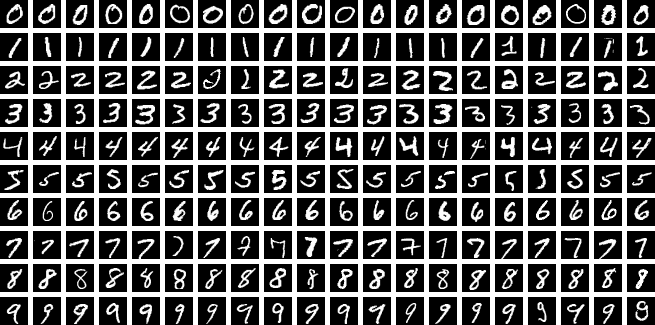
\includegraphics[width=0.8\linewidth]{MNIST_dataset_example.png}
    \caption{An example of MNIST digits \\
        Credit and source: User \texttt{Suvanjanprasal} at Wikipedia}
    \label{figExample}
\end{figure}
\newpage
\section{Implementation}
Given our four different methods, we have a branching code structured as follows:
\begin{figure}[ht!]
    \centering
    \includegraphics[width=0.5\linewidth]{generative.PNG}
    \caption{Our codebase}
    \label{figModel}
\end{figure}
\newline
We aim to keep all individual models as similar as possible. As such, every model, \texttt{[model].py} (eg. \texttt{GAN.py}) has a distinct two-part implementation, where we have one (or more) classes dedicated to the structure and behavior of the model, and one class solely dedicated to the actual training of the model. This in turn keeps our model flexible, universal within the confines of our overall project, and allows us to easily distinguish a given part of any single implementation.
\newline
More in depth, a given model and it's parameters is requested in \texttt{main.py} and passed to \texttt{runner.py}, which handles both the pre-processing of the data (together with \texttt{data.py}) and the optional retrieving of best (found) parameters in \texttt{usebest.py}. Should a non-optional parameter be left blank, a default value will be used, which are defined separately in each respective model.
\newline
We lastly have two separate scripts, \texttt{classify.py} and \texttt{plot.py}, which are relatively self-explanatory and relate more to testing of our model either mid-or post-training.
\newline
\texttt{plot.py} contains several functions, namely the plotting of ordered generated digits 0-9, plotting a random grid of generated digits, generating a \texttt{.gif} of the noise schedule over time steps and generating the evolution of a grid of generated numbers for each given time step and visualizing them as a \texttt{.gif}. We lastly also have a simple function that generates a grid at the first and final epoch.
\newline
\texttt{classify.py} is instead solely used to classify a given generated digit, within a confidence. This is so that we may order (and label) the digits plotted in \texttt{plot.py} where relevant, but also such that (if relevant) a user can request a given number, or a series of numbers.
\newpage
\section{Results}
For our results, the most relevant thing to be looking at is the evolution of our generative digits. As such, we will be looking at both the first and the final set of digits.
\newline
We start with RBMs
\subsection{Restricted Boltzmann Machines}
We let the script run for a total of 100 epochs, giving us:
\begin{figure}[ht!]
    \centering
    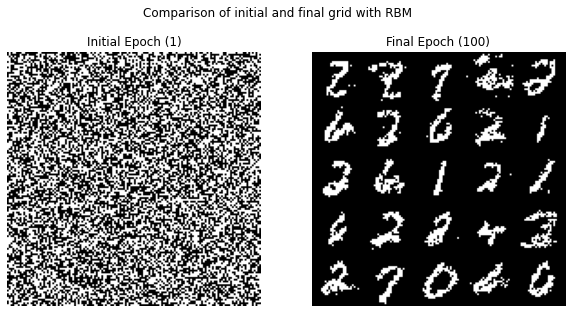
\includegraphics[width=0.7\linewidth]{RBM_first_final.png}
    \caption{25 generated digits in a 5x5 grid for our first and final epoch, respectively, with an RBM model. \newline
    Parameters: $n_{v} = 28\times28, \; \; n_h = 256, \; \; \eta = 2\times10^{-4}$
    \newline 
    A timelapse .gif can be found \href{https://github.com/simloken/Generative_Imaging/blob/main/Figures/RBM_evolution.gif}{here}}
    \label{figRBM}
\end{figure}
\newline
We see that our RBM model starts out initially as pure noise. There isn't even a hint of digits forming, however, at epoch 100 we can see digits forming, albeit poorly. Most of the digits are intelligible, with perhaps the exception being $\mathbf{1,4}$ and $\mathbf{5,4}$, the notation here being \textbf{row, column} respectively.
\newline
The results are perhaps to be expected. This is after all the most "primitive" of our tested methods, in the sense that it is the only non-traditional neural network.\newline
Another key take-away is that we definitely have no problems with overfitting. We see for example at $\mathbf{1,3}$ and $\mathbf{5,2}$ two distinct 7s. Likewise, we can see two distinct 2s in $\mathbf{4,2}$ and $\mathbf{5,1}$.
\newline
It is also worth pointing out that it is the only method that has a binary output. Any given pixel in the 28x28 grid have only two states, on or off, which gives the numbers a jagged look, whereas the other numbers will look as if they've had anti-aliasing applied to them.
\newpage
\subsection{Generative Adversarial Networks}
Next, we look at GANs
\begin{figure}[ht!]
    \centering
    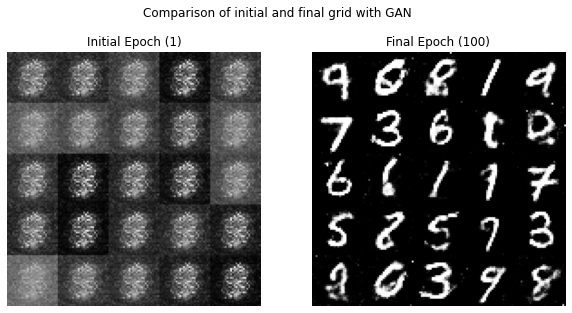
\includegraphics[width=0.7\linewidth]{GAN_first_final.png}
    \caption{25 generated digits in a 5x5 grid for our first and final epoch, respectively, with a GAN model. \newline
    Parameters: $\mathcal{D}_{L} = 100, \; \; \eta = 2\times10^{-4}$
    \newline 
    A timelapse .gif can be found \href{https://github.com/simloken/Generative_Imaging/blob/main/Figures/GAN_evolution.gif}{here}}
    \label{figGAN}
\end{figure}
\newline
The first key take-away here is that we are no longer dealing with pure noise at $e = 1$, instead it looks as if we have some weird aggregate of all numbers. Like with the previous RBM model, we have distinct digits forming at the final epoch. We note also immediately now the "anti-aliasing" taking place. This is of course because, as previously discussed, pixel-values for this model is no longer binary. This in turn makes digits appear to be more 'smooth', and allows different parts of the digits to be emphasized. \newline
We again can see clear distinction between numbers. The standout example here is probably the 7s found at $\mathbf{2, 1}$ and $\mathbf{3,5}$, which are two different valid ways of writing the number 7. \newline
However, we note also that there are some digits that look a bit odd. For example, $\mathbf{5,1}$, which is by far the worst digit produced by the model.
\newpage
\subsection{Variational Autoencoders}
Now we look at VAE:
\begin{figure}[ht!]
    \centering
    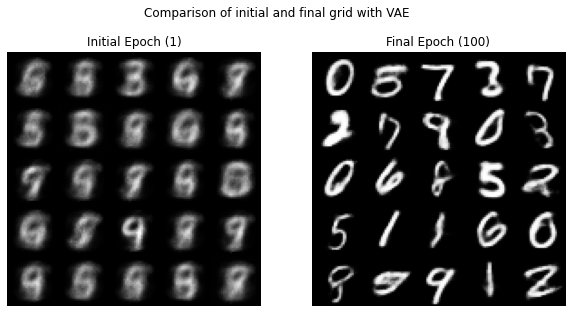
\includegraphics[width=0.7\linewidth]{VAE_first_final.png}
    \caption{25 generated digits in a 5x5 grid for our first and final epoch, respectively, with a VAE model. \newline
    Parameters: $\mathcal{D}_{L} = 100, \; \; \eta = 2\times10^{-4}$
    \newline 
    A timelapse .gif can be found \href{https://github.com/simloken/Generative_Imaging/blob/main/Figures/VAE_evolution.gif}{here}}
    \label{figVAE}
\end{figure}
\newline
Here, we see that like with the previous GAN model, we again have a pseudo-aggregate for our initial epoch. However, unlike the GAN, we can in some cases make out blurry attempts at digits, the standout being $\mathbf{4, 3}$. This suggests that the VAE converges much faster than our previous models. Looking at the final epoch, we see again good results. We see also distinct digits (again 7 is a good example with $\mathbf{1,3}$ and $\mathbf{1,5}$), with the only poor digit being the 9(?) found at $\mathbf{5,1}$, which looks more like an umbrella or a mushroom.
\newline
One thing that is also worth noting is that, unlike RBM and GAN, there is no visible noise for the final epoch, and digits are generally more "smooth" and "continuous" than it's previous counterparts.
\newpage
\subsection{Denoising Diffusion Probabilistic Models}
Finally, we look at our most advanced model, the DDPM:
\begin{figure}[ht!]
    \centering
    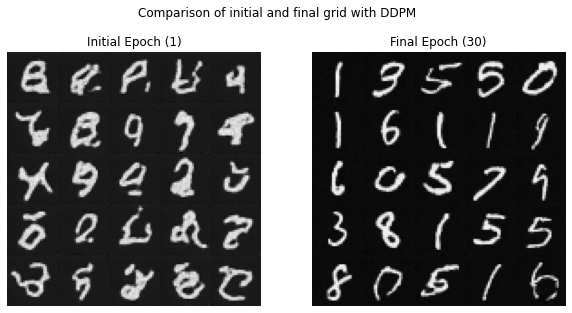
\includegraphics[width=0.7\linewidth]{DDPM_first_final.png}
    \caption{25 generated digits in a 5x5 grid for our first and final epoch, respectively, with a DDPM model. \newline
    Parameters: $t_n = 500, \; \; \beta_0 = 1\times10^{-4}, \; \; \beta_n = 2\times 10^{-2}, \; \;  \eta = 2\times10^{-4}$
    \newline 
    A timelapse .gif can be found \href{https://github.com/simloken/Generative_Imaging/blob/main/Figures/DDPM_evolution.gif}{here}}
    \label{figDDPM}
\end{figure}
\newline
The first thing that jumps out at us is the fact that the initial epoch is no longer an aggregate or pure noise, instead shaping up to be digits or digit-like, with some cases (like $\mathbf{1,1}$ or $\mathbf{2,3}$) being intelligible. This suggests that DDPM is an even faster learner than the previous methods. \newline
This is good, as DDPM is a much more computationally intensive method than the previous methods, and as such, we limit ourselves to 30 epochs. Looking at our final epoch, we see again very good and generally continuous digits, and very little if no noise. We see also distinct numbers, with differently oriented 8s in $\mathbf{4,2}$ and $\mathbf{1,5}$, and the different 6s in $\mathbf{2,2}$ and $\mathbf{5,5}$. 
\newline
We note also the excess of 1s. This could be a type of overfitting, but there is also no guarantee that we get an even spread of numbers, given the random nature of our model, noting also the total absence of 2.
\newpage
\section{Discussion}
\subsection{A quick overview of the results}
Perhaps the best way to quickly discuss and summarize the results would be to make a series of bullet points for a given model, now that we've both worked with and seen them in action.
\subsubsection*{RBM}
\begin{itemize}
    \item Conceptually straightforward
    \item Only model to not rely on traditional Neural Networks and its strengths
    \item Binary outputs
    \item Slow to train
    \item Relatively poor results
\end{itemize}
\subsubsection*{GAN}
\begin{itemize}
    \item The idea of two networks competing is relatively straightforward
    \item Requires tuning of two different networks
    \item Prone to produce noisy digits
    \item Relatively easy to implement
    \item Relatively good results
\end{itemize}
\subsubsection*{VAE}
\begin{itemize}
    \item Conceptual difficulty is midway between GANs and DDPMs
    \item Produces smooth, continuous digits
    \item Very easy to implement
\end{itemize}
\subsubsection*{DDPM}
\begin{itemize}
    \item Hardest to grasp conceptually
    \item Computationally heavy
    \item Complex to implement
    \item Perhaps a bit overkill for MNIST digits
    \item Relatively good results
\end{itemize}
\subsection{Objective measurement of model performance}
Although outside the span of this paper, the question remains if there is someway to objectively measure the performance of a given model. One might be tempted to compare losses across models, but recall that these are not uniform and thus might not be the same magnitudes, meaning such comparisons are useless.
\newline
An alternative may perhaps be to instead look at the quality of the generated digits. For example with a different classification network that determines whether or not a digit is "good". This would of course require extensive tuning, to ensure the classification network is neither too strict, nor too lenient, making it a delicate balancing act. 
\newline
However, if tuned correctly, this could give an objective measurement of all our models as to which is best suited for MNIST digits. \newline
Although, this would not necessarily take into count the complexity of the problem in relation to the complexity of the model. Like hinted at in the previous section, DDPM is perhaps a bit overkill for such a problem, especially when taking into account the relative complexity of implementing the model, as opposed to something simpler like GANs or VAEs. We can therefore make an argument that there isn't necessarily an objectively "best model", when looking at just model performance, but that we must instead weigh model complexity, problem complexity and results against each other.
\subsection{Applicability to Physics problems}
If you remember, we discussed briefly the applicability of generative imaging to scientific research as a motivator for our research. As a physics student at the Department of Physics, it is therefore perhaps most relevant to now spend some time discussing more at length the applicability specifically to physics problems. \newline
One particularly prominent example that was not previously mentioned is CaloGAN \cite{Paganini_2018}, which is notable for being a prominent example of applying generative imaging techniques to high-energy physics simulations. \newline
In short, in high-energy physics, detailed simulations of particle interactions and energy depositions in detectors (like calorimeters) are computationally expensive with traditional methods. CaloGAN leverages a GAN to create realistic simulations of electromagnetic and hadronic showers in multi-layer calorimeters, showing an incredibly promising alternative that significantly lowers the computational burden while maintaining fidelity to the physics processes.
\subsection{Further improvements}
One obvious point of discussion is what we could improve on with our model, besides the obvious like digit fidelity or runtimes. \newline
One possible venue of improvement could be to extend the possible numbers of digits in a number from one to two or even three. This could be done by levying the existing MNIST dataset, and combining random digits to form new numbers. Of course, some modifications would need to be made to the individual digits, such as removing the rightmost and the leftmost pixels of two digits such that it looks like a natural, human-drawn number, and not just two digits spliced together. With such a dataset, we can then train our network to create multi-digit numbers, albeit at an increased computational, complexity and tuning cost.
\subsection{Thoughts regarding the topic}
Last I wish to share some of my thoughts regarding this topic of research, and if I'd recommend it. \newline
I found the topic to be interesting, especially the many different approaches to generative imaging that I've studied. Of all methods, I believe VAE to be my favorite both in terms of how lightweight it was, but also how straight-forward and easy it was to implement in relation to its power as a generative method. Of course, it is impossible for me to say as of right now whether this method is scalable to more complex databases like animals, faces or the like, and I believe this could be an interesting topic - rather than focusing on introducing many different methods, one may focus on just one method and attempt to push it to its limits, given a sufficient dataset. One quick look on Kaggle reveals both datasets for cats \footnote{https://www.kaggle.com/datasets/borhanitrash/cat-dataset} \footnote{https://www.kaggle.com/datasets/crawford/cat-dataset} and dogs \footnote{https://www.kaggle.com/datasets/jessicali9530/stanford-dogs-dataset}, which could prove to be an interesting challenge in sufficiently generating new images. \newline
I would therefore wholly recommend this or an adjacent topic should anyone have any interest at all, as it is an emerging field with many interesting possibilities. 
\newpage
\section{Conclusion}
We have shown in this work the fundamentals of generative imaging, and we have provided an introductory examination of four generative imaging methods: RBMs, GANs, VAEs and DDPMs, demonstrating their capacity to generate new instances of MNIST digits. Each method, which are entirely unlike each other, contributes uniquely to our understanding of the generative processes in neural architectures. Collectively, the models not only underscore the rich diversity of possible approaches, but help pave the way for future research that may integrate or further refine these methods. Future work could explore hybrid models, or applications to more complex datasets to continue advancing the field of generative imaging.
\newpage
\bibliographystyle{unsrturl}
\bibliography{citations.bib}
\newpage
\end{document}
